%!TEX root = ../masters.tex

\chapter{Metodologia}
\label{cha:metodology}

\section{Escolha do Corpus}
\label{sec:corpus}

\section{Desenho do Experimento}
\label{sec:experiment-design}

\section{Ambiente Tecnológico}
\label{sec:tech-environment}

Este trabalho tem como metodologia uma pesquisa de caráter não-experimental e quantitativa, por se tratar de coleta de informações e comparação de resultados de técnicas de extração de metadados em artigos científicos.

Desta maneira, a pesquisa de modo padrão não traz alteração nos ambientes pesquisados, apenas os analisa e os compara com base em padrões estabelecidos como sendo de resultado adequado. Assim, o projeto em si trata muito mais de pré-seleção de documentos e técnicas a serem testadas como também dos resultados já analisados e que são necessários para uma técnica ser considerada produtiva.

% Explicar o passo a passo que será utilizado

Primeiramente, são filtradas as técnicas encontradas a fim de analisar realmente as que são necessárias dentro do objetivo da pesquisa, fazendo do projeto o mais conciso possível. Desta forma, diversos elementos serão utilizados a fim de se obter os resultados desejados. Os elementos se relacionam entre si e estão identificados na \autoref{fig:metodology}. 

% Colocar diagrama demonstrando a relação entre todos os objetos, como artigos, técnicas, o processamento, a planilha de resultados e as conclusões

\begin{figure}
    \centering
    \caption{Processo de Metodologia}
    \label{fig:metodology}
    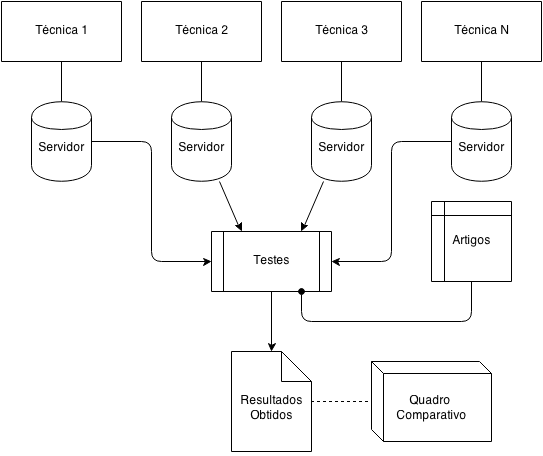
\includegraphics[width=0.7\linewidth]{./assets/images/metodology}
\end{figure}


\section{Seleção das Técnicas/Ferramentas}
\label{sec:choosen-tools}

As técnicas que foram analisadas dentro do capítulo de \textbf{Revisão de Literatura} compreendem um universo atuante e de caráter livre, independente da linguagem de programação que foi utilizada no desenvolvimento, exceto pelos detalhes explicados nas limitações do trabalho.

Em função do grande número de ferramentas disponíveis como resultado desta pesquisa, algumas foram selecionadas a fim de se obter ao máximo os testes e os resultados esperados.

Conforme mencionado anteriormente, ferramentas pagas ou que não disponibilizam o código para instalação não foram testadas, visto que a necessidade do atual trabalho visa identificar os resultados obtidos dentro de um conjunto de infra estrutura única, de maneira justa com cada projeto.

Assim sendo, a \autoref{tab:tools} lista as seguintes ferramentas que foram selecionadas para teste dentro do escopo proposto neste trabalho.

% Colocar uma tabela com as técnicas que serão comparadas

\begin{table}
    \caption{Ferramentas selecionadas para testes}
    \begin{center}
    	\begin{tabular}{|p{6cm}|p{5cm}|}
			\hline \textbf{Ferramenta} & \textbf{Linguagem} \\ 
			\hline Ferramenta 1 & Java\\
			\hline Ferramenta 2 & Perl\\
			\hline Ferramenta 3 & Python\\
			\hline Ferramenta 4 & Java\\
	    	\hline 
    	\end{tabular} 
    \end{center}
  	\label{tab:tools}
\end{table}

\section{Seleção de Artigos}

Visando provar a eficiência destas técnicas, desejamos ter informações de saída consideradas corretas para que seus resultados possam ser comparados e verificados com exatidão. Assim, foi selecionada uma série de artigos científicos das mais diversas áreas de pesquisa, de diversos eventos distintos, com padrões visuais totalmente diferentes e que são possível de ser analisados e coletados.

% Áreas dos Artigos e Eventos

Desde modo a lista destes artigos compreende um total de 100 documentos variados, com seus metadados já extraídos manualmente e todos catalogados a fim de ter o resultado da aplicação das técnicas comparado com os resultados obtidos manualmente. Na \autoref{tab:papers-list} pode-se ver o número de artigos que foram selecionados por cada área do conhecimento. A relação de todos os artigos analisados pode ser obtida no \autoref{appendix:papers} deste documento.

Os artigos foram selecionados tomando como base a principal forma de análise das técnicas selecionadas para testes: o layout, ou seja, a disposição dos elementos nos artigos científicos. Esta seleção foi feite com base a abranger um maior número de representações, com disposições diferentes, tipografias diferentes e inclusive ordem diferentes nas exibições. Desta forma as técnicas poderão ser confrontadas e os resultados comparados com os resultados esperados.

% Artigos em Inglês, somente

Todos os artigos selecionados foram escritos na língua inglesa. Esta decisão foi tomada em virtude de além de ser a língua inglesa universal para disseminação de conhecimento, ela é a mais utilizada no meio acadêmico, de maneira a ter um universo muito maior de artigos escrito em inglês do que outras línguas.

Além disso a abrangência de outros idiomas entraria em um aspecto que não é objetivo deste trabalho abordar, visto a diversificação de culturas e símbolos, fazendo com que línguas orientais, como o mandarim ou japonês, tenham análises diferenciadas em função de suas diferenças na forma de representação.

\begin{table}
    \caption{Seleção de artigos científicos para testes (ainda em desenvolvimento)}
    \begin{center}
        \begin{tabular}{|l|l|}
        	\hline
            \textbf{Área de Conhecimento} & \textbf{Total de Artigos} \\ 
            \hline
            Arquitetura e Urbanismo & 7 \\ 
			Música & 7 \\ 
			Ciência da Computação & 8 \\
			Ciência da Informação & 9 \\
            Ciências Biológicas & 7 \\
            Direito & 7 \\
            Engenharia Civil & 8 \\
            Letras & 7 \\
            Matemática Computacional & 7 \\
            Medicina & 9 \\ 
            Odontologia & 8 \\ 
            Psicologia & 9 \\
            Sociologia & 7 \\	
            \hline
            \textbf{Total} & \textbf{100} \\
            \hline 
        \end{tabular}
    \end{center}
    \label{tab:papers-list}
\end{table}

\section{Infraestrutura Computacional}
\label{sec:computational-structure}

Para que os testes sejam feitos de maneira adequada e independente, sem interferência de outras técnicas nos resultados, serão utilizados N servidores, sendo N o número total de técnicas a serem avaliadas.

Deste modo, para cada técnica avaliada será configurado um servidor com as linguagens de programação necessárias e todos os pré-requisitos que a técnica necessita para funcionar. Estes servidores serão definidos através de máquinas virtuais, o que traz benefícios não somente de performance mas de flexibilidade quanto das tecnologias necessárias para o funcionamento de cada técnica.

\subsection{Testes In Logo}
\label{ssec:in-loco-tests}

% Falar de técnicas que já possuem algum site para testes, demonstrando a ferramente funcionando

Algumas técnicas de extração de metadados disponibilizam acesso online a uma ferramenta gratuita para testes. Deste modo, para estes casos específicos não será necessária a criação de servidores e instalação dos pacotes, visto que o ambiente de testes poderá ser feito dentro da ferramente fornecida pelas desenvolvedoras das técnicas.

% Vantagem de ser feito o teste online

Este fato garante uma maior precisão nos resultados, inclusive pelo fato de o ambiente de testes estar 100\% funcionando e ter sido disponibilizado pela mesma equipe de desenvolvedores do projeto, garantindo a eficácia nos resultados que essa técnicas fornece.

\section{Quadro Comparativo}
\label{sec:comparative-board}

Visando uma comparação dos resultados eficaz todos os resultados serão inseridos em um documento formato planilha para serem comparados manualmente e as conclusões então obtidas. Para tal esta planilha de resultados a chamaremos de 'Quadro Comparativo" e será exclusiva para comparação dos resultados das técnicas analisadas.

% Formato online para consulta futura

Com o objetivo de facilitar o acesso às informações este documento é disponibilizado como anexo deste projeto e ainda tem seu acesso liberado em formato online. Desta forma qualquer pessoa poderá ter acesso aos resultados obtidos pelos testes e comparar elas mesmas os dados contidos na planilha.

\section{Metadados, Pesos e Resultados}
\label{sec:metadata-results}

% Importância de se ter pesos em função dos metadados

A extração de metadados de artigos científicos engloba um processo onde os resultados obtidos, mais especificamente os metadados propriamente ditos, possuem características diferenciadas que podem influenciar em uma busca por artigos, feita por um pesquisador.

Desde modo atribuímos pesos para cada um dos metadados analisados, de maneira a identificar os mais importantes e que podem contribuir com um número maior de resultados de busca. 

% Quais metadados são mais importantes para uma pesquisa de artigos

Alguns metadados são mais importantes que outros no que diz respeito à funcionalidade de pesquisa. Geralmente quando vamos buscar artigos, seja na Internet, ou em algum outro local, geralmente buscamos primeiro pelo título do artigo (quando procuramos por um artigo em específico) ou então pelo nome do autor (quanto procuramos artigos de um determinado autor).

Além disso, utilizamos também o título, juntamente com o resumo, para buscar de palavras chaves ou palavras que podem ser relevantes na pesquisa pelos documentos. Assim sendo alguns metadados devem ser mais considerados no resultado destas extrações, por serem mais importantes no ponto de vista da busca.

Assim sendo apresentamos a \autoref{tab:metadata-weight}, que demonstra como cada metadado teve sua importância interpretada e qual o peso que lhe foi atribuído, sendo utilizado o inteiro 1 para o peso mais baixo e o 5 para peso mais alto, sendo consequentemente o mais importantes.

% Tabela de metadados e pesos

\begin{table}
    \caption{Os metadados e seus pesos atribuídos}
    \begin{center}
    	\begin{tabular}{|p{3cm}|p{8cm}|C{1cm}|}
			\hline \textbf{Metadado} & \textbf{Relevância} & \textbf{Peso} \\ 
			\hline Título & Um dos termos mais buscados quando se pesquisa um artigo & 5 \\
	    	\hline Autor(es) & O segundo termo mais pesquisado & 4 \\
	    	\hline E-mail(s) & Pouco relevante no quesito pesquisa de artigos & 1 \\
	    	\hline Resumo & Importante por conter palavras chaves e o resumo propriamente dito & 3 \\
	    	\hline Referências & Muito importante e necessário, pois será utilizada na referência inversa de autores & 5 \\
	    	\hline 
    	\end{tabular} 
    \end{center}
  	\label{tab:metadata-weight}
\end{table}

% Falar sobre a porcentagem de acertos em cada metadado, por exemplo, se o resultado extraiu 90\% do resultado (não a totalidade), deve ser considerado um valor para este resultado, não somente sim ou não.

Outro detalhe importante é a precisão de cada resultado para cada metadado analisado. Em alguns casos o título, por exemplo, não é extraído em 100\% mas alguma variação dele. 

Deste modo consideramos 3 (três) resultados possíveis para um resultado analisado:

\begin{enumerate}
    \item \textbf{Preciso:} Quando um resultado atinge acima de 95\% de precisão, ou seja, o campo foi extraído em 95\% ou mais de sua totalidade.
    \item \textbf{Satisfatório:} Quando um resultado atinge entre 90 e 94\%, o que pode ser considerado satisfatório e a maioria do conteúdo consegue ser analisada sem maiores problemas.
    \item \textbf{Inaceitável:} Quando o resultado atinge abaixo de 90\%, ou seja, entre 0\% e 89\%. Este resultado no âmbito do presente projeto é considerado inaceitável.
\end{enumerate}

Assim, temos o valor de cada resultado possível, que será também utilizado no processo de análise, conforme consta na \autoref{tab:precision}. Cada valor, independente de sua classificação será utilizado para o cálculo final da nota de cada ferramenta.

% Tabela de precisão e os valores

\begin{table}
    \caption{Resultados obtidos em cada metadado e sua precisão}
    \begin{center}
    	\begin{tabular}{|C{3cm}|C{3cm}|}
			\hline \textbf{Resultado} & \textbf{Precisão} \\ 
			\hline Preciso & 1\\
	    	\hline Satisfatório & 0.60 \\
	    	\hline Inaceitável & 0 \\
	    	\hline 
    	\end{tabular} 
    \end{center}
  	\label{tab:precision}
\end{table}

\subsection{Índice de Confiabilidade}
\label{ssec:confiability-index}

% Fórmula final para a nota final de cada técnica

Considerando que cada metadado possui um peso diferente necessitamos calcular o índice de acertos a ser utilizado em cada resultado coletado para cada técnica aplicada. Assim sendo chegamos em uma fórmula matemática à qual chamamos ''Índice de Confiabilidade'', que calcula o resultado obtido através dos pesos que foram atribuídos a cada campo.

Este índice utiliza os pesos anteriormente definidos e a precisão dos resultados obtida, de maneira a permitir chegar em uma única nota final para cada técnica aplicada.

Basicamente a fórmula atua como uma média ponderada dos resultados alcançados na extração de cada campo do artigo, seguindo os pesos apresentados em \autoref{tab:metadata-weight}. Cada peso é atribuído ao resultado encontrado em cada ferramenta testada. 

A título de exemplo, após o teste de uma ferramenta, supondo que ela conseguiu extrair 87\% dos títulos dos artigos com sucesso, sua precisão com relação ao título será 87, que será multiplicado pelo peso correspondendo ao seu campo, neste caso, o inteiro 5. Isso ocorre para todos os campos apresentados, seguindo seus respectivos pesos.

A descrição de cada variável no Índice de Confiabilidade poderá ser obtida de acordo com a \autoref{tab:confiability-index}, onde temos as variáveis que fazem parte da fórmula descrita.

\begin{center}
	$ IC=\frac{5(PT)+4(PA)+PE+3(PR)+5(PRF)}{18} $
\end{center}

\begin{table}
    \caption{Descrição de cada variável no Índice de Confiabilidade}
    \begin{center}
    	\begin{tabular}{|p{3cm}|p{8cm}|}
			\hline \textbf{Variável} & \textbf{Descrição}\\ 
			\hline PT & Precisão na obtenção do título \\
			\hline PA & Precisão na obtenção do(s) autor(es)\\
			\hline PE & Precisão na obtenção dos e-mails dos autores \\
			\hline PR & Precisão na obtenção do resumo \\
			\hline PRF & Precisão na obtenção das referências \\
	    	\hline 
    	\end{tabular} 
    \end{center}
  	\label{tab:confiability-index}
\end{table}


